\documentclass{article}
\usepackage[utf8]{inputenc}

\title{Polarity Detection of Financial News}
\author{ John Michael Kovachi }
\date{April 16th, 2018}

\usepackage{graphicx}
\usepackage{listings}

\begin{document}

\maketitle

\section{Introduction}

    Natural language processing (NLP) has made the prospect of analysis of large financial corpora a reality. Analyzing financial texts for detection of sentiment is a particularly strong area of interest in the current NLP landscape. Correct classification of financial news has practical applications, including uses such as predicting stock price movements for publicly traded stocks. Traditional methods of sentiment analysis include detecting explicit sentiment in subjective corpora such as Twitter messages. Financial news texts, however, are not always explicitly subjective but often contain implicit polarity statements. Therefore, sentiment analysis and polarity detection of financial texts has required innovation of new techniques in order to obtain better results. 
    
    Recent efforts in this field have included the use of traditional linear classifiers, like the ones used in this paper, to the introduction of deep learning and word embedding techniques. Luss and D'Aspremont (2012) used a support vector machine and bag of words features to classify financial news articles. Their linear SVM showed that predicting absolute returns from financial news articles performs optimally when using articles that were released before approximately 10 AM. This SVM achieved a classification rate of 63 percent. Additionally, Luss and d'Aspremont used a multiple-kernel learning framework to produce an SVM that achieved a classification accuracy of up to 71 percent. Ding et al use a deep learning method for event-driven stock prediction (2015). Several models were tested, the most successful being a deep convolutional neural network using the aforementioned event-driven feature representation. This model performed with an accuracy of 65.48 percent on prediction of individual stocks. Peng and Jiang (2017) developed a number of different classification techniques in order to evaluate the Reuters dataset, including using price, point-wise mutual information, bag-of-keywords, and structured event word embeddings similar to Ding et al in their feature set. Peng and Jiang achieved a minimum error-rate of 43.13 percent using these methods. This corresponds with 
        
    In this paper, we will look at a large financial news corpus and perform classification on time-series data ranging over a number of years. We will look at a small set of companies, with hopes of expanding this set in future research. For now, we will focus on using a set of linear classifiers and a lexicon based method, with hopes of expanding to neural-network based method in the future.

\section{Methodology}
    The corpus used for information extraction was the Reuters corpus (Ding et al 2015). The corpus contains over 100,000 news articles from the years 2006-2013 covering a wide variety of topics in the financial domain. Each article was preprocessed before insertion into MongoDB, a NoSQL document database holding each document and its related metadata, including article date, article title, and a link to the article. Multiple training and classification methods were used to compare performance using different algorithms.  
    
    \begin{figure}
        \centering
        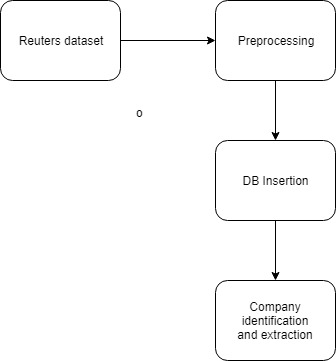
\includegraphics[scale=0.5]{Extraction.jpg}
        \caption{Preprocessing and data extraction in process}
        \label{fig:my_label}
    \end{figure}
    
    \subsection{Stock Price Querying}
    Stock price movements were queried using the Quandl API. The Quandl WIKI dataset, which contains stock price information for over 3,000 major US companies, was used for querying has stock price information.  The article date included in the metadata was used to query the API for stock price movements corresponding to a certain date. The WIKI dataset has historical prices dating back to 1997, and has date-range queries. Date-range queries were used to determine stock price changes over the course of a time specified by training or classification methods. Quandl queries occurred using REST API GET request. An example Quandl API call is including in the figure below.
    
    \begin{figure}
        \centering
        \includegraphics{}
        \caption{Caption}
        \label{fig:my_label}
    \end{figure}
    
    \subsection{Companies}
    A set of 30 companies were used to detect and train classification on. If a company was detected to exist in an article title, the article was used in the classification step. If no companies were detected in the article title, that article was discarded. Initially, named entity recognition was used to detect companies but this was determined to be too inaccurate to use for classification. Another method attempted was to use regular expressions to parse company names from a master list of company names provided from the WIKI dataset. This proved unreliable because the varying nature of the spelling of somme companies. For example, a company such as "JP Morgan" may be spelled as "J.P. Morgan" in a headline, and an exact string match would fail to identify the company in the headline. Therefore, only companies with clearly distinguishable, unvarying names such as "Lyondellbasell" or "Honeywell" were used in the company extraction, training, and classification process.  Future research may involve accurately detecting companies in order to perform analysis on a larger number of companies. 
    
    \subsection{Training}
    
    For training, several classification methods were used. First, a rudimentary lexicon method was used to determine the polarity of a specific article. Each sentence was in the article was tokenized, and subsequently each word in the article was tokenized and lemmatized. The McDonald financial sentiment word lexicon (2014) was used to count the number of positive and negative word occurrences in an article. If positive words outnumbered negative words, the article would be labeled as positive and vice versa. It should be noted that only sentences in the article that referenced the company extracted in the title were used for classification. This method was tested against stock price query returns for 1 day after the article was published, 2 days after the article was published, and a week after the article was published.
    

    
    Next, a multinomial Naive-Bayes classifier was used to classify articles. For training, a subset of the Reuters articles were used to provide gold standard labels. The Sem-eval subtask 5 training dataset was used for training this algorithm. This training data utililizes over 1000 financial news headlines that have each have a labeled score from -1 to 1. A score of -1 indicates the headline is bearish, while a score of 1 implies the headline is bullish. A bearish headline was therefore interpreted to have a negative polarity while a bullish headline was interpreted to have a positive polarity. Headlines with labels between -0.25 and .25 in polarity were not used, because these labels indicated a neutral headline. Therefore, headlines with a -1 to -0.25 label were given the class label "negative" while labels with a polarity from .25 to 1 were given a class label "positive".  This training set was then used to train the Naive Bayes classifier. The Naive Bayes classifier used was from NLTK's classification library. The Naive Bayes algorithm employs a bag-of-words model, meaning feature extraction is agnostic to position. Obtaining a probability of word w given a class c involves taking a count of w in all documents in the set and then taking a count of all words belonging to the given class in the document. Again, only sentences in articles that referenced a company extracted from the title of the article were selected to enter our bag of words model. 
    
    \begin{lstlisting}[caption={An example of a training object from the Sem-Eval task 5 dataset.}]
    
    
    {
        "id": 73,
        "company": "Barclays",
        "title": "World's banks may halve jobs and branches within 10 years - 
                    Barclays ex-boss",
        "sentiment": -0.521
    }
    
    
    \end{lstlisting}
    
    \medskip
    
    \begin{math}
    (1) \quad  P(w_i | c) = \frac{Count(w_i | c) + 1}{(\sum_{w \epsilon  V} Count(w | c)) + |V|}
    \end{math}
    
    \medskip
    
    A loglikelihood is applied to (1) for each feature. Classification utilized the $argmax_{c \epsilon C}$ for all classes available (in this instance, just the positive and negative class) (Jurafsky 2017). 
    
    \medskip
    
    Finally, an SVM (support vector machine) classifier is introduced. This SVM is a part of Scikit-learn's classification library. The features used in the SVM were vectorized using a vectorizer module and had term-frequency inverse-document-frequency (Luss, D'Aspremont 2012) applied to them in order to give a weight to the words in the corpus. The SVM was trained in two ways. First, it was trained on text features extracted from the body of text of each article. Second, it was trained on text features extracted from the titles of each article. An SVM is an optimization function that plots points in n-dimensional space. The primary goal of the SVM is to optimize a hyper-plane to best create distinctions between multiple classes in n-dimensional space. To determine class-labels for the SVM, a slightly different methodology was used compared to the MN Naive-Bayes classifier. Stock price movements were used to give class labels to each article in the training set. (While collecting articles to be used in the training set, every fourth article was used in the test set. This article was not used in the test set. Accordingly, approximately 75 percent of articles were used in the training set, and 25 percent were used in the test set). To determine the class label for a given document, the Quandl API was queried using an initial date and a later date (1 day later, and 1 week later). The later date stock price is compare against the initial date, in a ratio expressed here:
    
    $
    \frac{Price_{later}}{Price_{initial}}
    $
    
    If this ratio is $<= .985$ we apply a negative class label to the article. If the ratio is $>= 1.025$, we apply a positive label to the article. The thresholds picked are arbitrary, but represent an approximation for negative or positive movements in a given stock. These labels are applied to the training set, and are subsequently used for classification. Refer to the figure below a visualization of the SVM training process.
    
    
    
    \begin{figure}
        \centering
        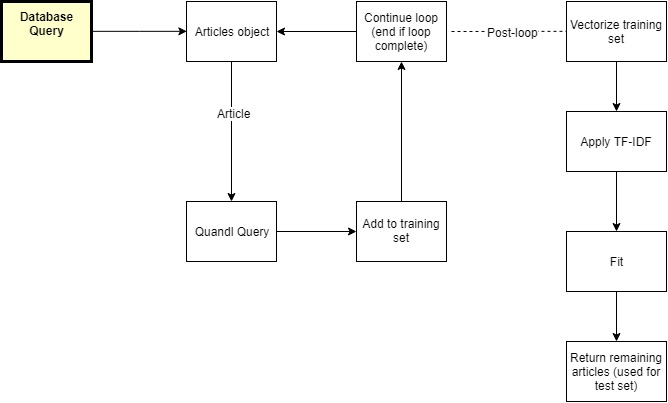
\includegraphics[width=\linewidth]{SVMtraining.jpg}
        \caption{SVM training process diagram}
        \label{SVM training}
    \end{figure}
    
    \subsection{Classification}
    
    The test articles used were disjoint from the training articles in order to prevent problems of overfitting. To make a classification decision, each method was used (lexicon, NB, SVM) and to obtain a class (positive, negative) for each article. This decision was then referenced against the Quandl API query. If the price movement for the day was positive, then the decision must be positive for an accurate decision. If the decision was negative yet the price movement was positive, then the classification decision was incorrect. This same process was used, conversely, for the negative class, where a negative price movement and negative decision was labeled correct, and negative price movement but positive decision was incorrect. Precision, recall, and F-Score was then obtained from these results. Price movements were used as a gold standard for classification because they were determined to be the best proxy for simulating real trading. Additionally, annotating a large amount of data was out of the scope of this project. In future research, annotated labels will be applied to training and testing data, in order to acquire more consistent methods of training the classifier and obtaining consistent results. 
    
\section{Results}

    Results varied depending on the classification methods used. For a two-day prediction threshold, the SVM classifier classified the documents at an accuracy of 54.6 percent. For a one-week threshold, the classifier classified 53.2 percent. For the Naive Bayes classifier, we obtained an accuracy of _ on the documents with the two-day prediction threshold. For the one week threshold, we obtained an accuracy of _ on the documents. 
    


\section{Discussion}

    Results varied depending on the classification methods used. 

\section{Future Research}
    
    As mentioned earlier in the article, several avenues of future research could potentially improve results. Firstly, company identification is an open problem that could be solved by training an NER on a domain-specific dataset. This dataset would be annotated with company labels in order to train a maximum entropy classifier. This classifier could be used to perform the NER. Improvement in classification of company names could result in an overall improvement in training and would allow for a larger dataset to be trained and tested on. 
    
    Another area of research to be explored is the annotation of a larger amount of data than was used here. *Insert article* mentions a fine-grained annotation scheme that could potentially improve the features available to our classifier. Even standard polarity labels on a large number of documents could potentially improve accuracy. Labeling a large amount of data was out of the scope of this paper.
    
    Dependency parsing of sentences could be another method of classification. Linking entities and polarity words (referenced from a lexicon) in a dependency parsing tree on the sentence level could be used as a straightforward method of company stock prediction. It could also be used as feature input into a classifier.
    
    Finally, a non-linear deep learning model, as shown to have success in some of the papers mentioned earlier, including Ding et al, could potentially improve accuracy of classification. Event-driven feature representation in deep learning models have shown to have success in this specific classification problem, and future research in the subject could explore refinement in feature selection with this model.

\section{Sources}
        Note: this is a rough draft of the sources I have so far. Links will just be copied for now.
        
        http://www.aclweb.org/anthology/N16-1041 \newline
        https://www.ijcai.org/Proceedings/15/Papers/329.pdf \newline
        https://web.stanford.edu/~jurafsky/slp3/ \newline
        https://www.nltk.org/
        https://www.tandfonline.com/doi/full/10.1080/14697688.2012.672762?scroll=top&needAccess=true (Russ, D'Aspremont)
        https://www3.nd.edu/~mcdonald/Word_Lists.html (McDonald Word List)
    
\end{document}
